\documentclass[english]{beamer}
\usepackage[utf8]{inputenc}
\usepackage{url}
\usepackage[english]{babel}
\usepackage[T1]{fontenc}
%\usepackage[math]{iwona}
%\usefonttheme{professionalfonts}
\usepackage{amsmath}
%\usepackage{pplx}
%\usepackage{fontspec}
\setbeamerfont{note page}{family*=pplx,size=\footnotesize} % Palatino for notes
\setcounter{tocdepth}{1}
\usepackage[scaled]{helvet}
\renewcommand\familydefault{\sfdefault} 
\usepackage[T1]{fontenc}

\date{2019-01-09}


\definecolor{NavyBlue}{RGB}{0,0,128}

\setbeamercolor{normal text}{fg=white,bg=NavyBlue!90}
\setbeamercolor{structure}{fg=white}

\setbeamercolor{alerted text}{fg=red!85!black}

\setbeamercolor{item projected}{use=item,fg=black,bg=item.fg!35}

\setbeamercolor*{palette primary}{use=structure,fg=structure.fg}
\setbeamercolor*{palette secondary}{use=structure,fg=structure.fg!95!black}
\setbeamercolor*{palette tertiary}{use=structure,fg=structure.fg!90!black}
\setbeamercolor*{palette quaternary}{use=structure,fg=structure.fg!95!black,bg=black!80}

\setbeamercolor*{framesubtitle}{fg=white}

\setbeamercolor*{block title}{parent=structure,bg=black!60}
\setbeamercolor*{block body}{fg=black,bg=black!10}
\setbeamercolor*{block title alerted}{parent=alerted text,bg=black!15}
\setbeamercolor*{block title example}{parent=example text,bg=black!15}


\usetheme{Boadilla}
\useoutertheme{infolines}
\setbeamerfont{section in head/foot}{family=\sffamily}
\setbeamerfont{subsection in head/foot}{family=\sffamily}
\setbeamerfont{title in head/foot}{family=\sffamily}
\setbeamerfont{author in head/foot}{family=\sffamily}
\setbeamerfont{date in head/foot}{family=\sffamily}
\setbeamerfont{institute in head/foot}{family=\sffamily, size=\tiny}
\setbeamerfont{block title}{family=\sffamily}
\setbeamerfont{block title alerted}{family=\sffamily}
\setbeamerfont{block title example}{family=\sffamily}
%\renewcommand{\familydefault}{\rmdefault}











\definecolor{foreground}{RGB}{255,255,255}
\definecolor{background}{RGB}{24,24,24}
\definecolor{title}{RGB}{107,174,214}
\definecolor{gray}{RGB}{155,155,155}
\definecolor{subtitle}{RGB}{102,255,204}
\definecolor{hilight}{RGB}{102,255,204}
\definecolor{vhilight}{RGB}{255,111,207}

\setbeamercolor{titlelike}{fg=title}
\setbeamercolor{subtitle}{fg=subtitle}
\setbeamercolor{institute}{fg=gray}
\setbeamercolor{normal text}{fg=foreground,bg=background}

\setbeamercolor{item}{fg=foreground} % color of bullets
\setbeamercolor{subitem}{fg=gray}
\setbeamercolor{itemize/enumerate subbody}{fg=gray}
\setbeamertemplate{itemize subitem}{{\textendash}}
\setbeamerfont{itemize/enumerate subbody}{size=\footnotesize}
\setbeamerfont{itemize/enumerate subitem}{size=\footnotesize}



\begin{document}

\title{Personalens inst{\"a}llning till uppf{\"o}ljning och screening via patientens smartphone, exemplifierad av ett fr{\aa}geformul{\"a}r f{\"o}r sj{\"a}lvbed{\"o}mning av depressionssymptom.}
%\author[ABC]{ABC\\[5mm]{\footnotesize \textbf{Supervisors:}\\Prof. QWERTY\\Prof. DEF GHI\\Prof. Jklmno Pqrst\\}}
\author[]{F{\"o}rsta f{\"o}rfattare: Rickard Hultgren\newline Handledare: Mikael Sandlund\newline Bihandledare: Helj{\"a} Pihkala}
%\url{http://slackware.com/~alien/}\\
%\texttt{alien@slackware.com}

\institute{\\
{\fontfamily{ptm}\selectfont{
UME{\AA} UNIVERSITET\\
%\url{http://umu.se/}
}}
}

\begin{frame}
	\titlepage
\end{frame}


\section{Overview}
\begin{frame}
	\frametitle{Statistik i psykiatri}

	\begin{itemize}
	\item 50--80\% av beg{\aa}ngna suicid {\"a}r associerade med affektiva sjukdomar.
	\item Suicid {\"a}r den fr{\"a}msta orsaken till d{\"o}dsfall bland m{\"a}n mellan 15 och 44 {\aa}r i Sverige.
	\item 2/3 av alla suicid nyligen hade varit i kontakt med v{\aa}rden.
	\end{itemize}

	\pause

	\textit{Slutsats:\\Patientens affektiva tillst{\aa}nd f{\"o}rst{\aa}s inte alltid av l{\"a}karen.}\\\ \\

\pause

L{\"a}karens fel?\\
Patientens fel?\\
D{\aa}liga verktyg f{\"o}r kommunikation?
\end{frame}

\subsection{}
\begin{frame}
\ \\ 
eMADRS {\"a}r en app f{\"o}r android som best{\aa}r av ett digitalt MADRS-S formul{\"a}r. Resultatet skickas via SMS till angivet nummer.\\\ \\

Att utl{\"a}sa fr{\aa}n MADRS-S resultat:
	\begin{itemize}
	\item allvarighetgraden av symptombilden.
	\item MADRS-S ger ej diagnos.
	\end{itemize}
K{\"a}llkod:\\
\href{https://github.com/RickardHultgren/emadrs}{\url{https://github.com/RickardHultgren/emadrs}}\\
Nedladdning:\\
\href{https://play.google.com/store/apps/details?id=rickardverner.hultgren.emadrs}{\url{https://play.google.com/store/apps/details?id=rickardverner.hultgren.emadrs}}

\end{frame}

\subsection{}
\begin{frame}
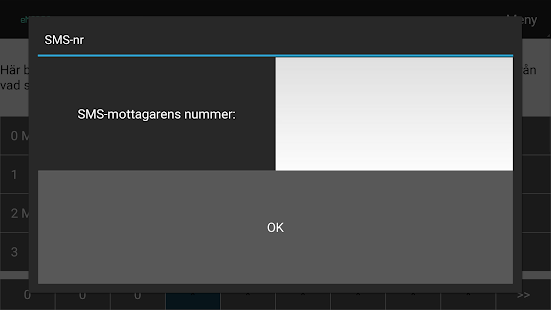
\includegraphics[scale=0.4]{1.png}
\end{frame}

\begin{frame}
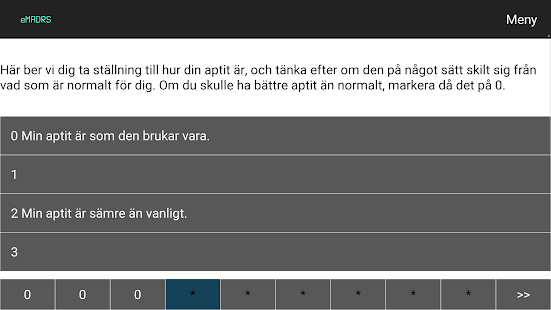
\includegraphics[scale=0.4]{2.png}
\end{frame}

\begin{frame}
\frametitle{Fr{\aa}gest{\"a}llningar}
	\begin{itemize}
	\item Vilka f{\"o}rdelar och nackdelar identifieras ur ett professionellt kliniskt perspektiv, med att anv{\"a}nda ett digitalt utv{\"a}rderingsinstrument f{\"o}r depression i screening och uppf{\"o}ljning?
	\item F{\"o}rslag till vidareutveckling av eMADRS.
	\item Vilka personalkategorier skulle p{\aa}verkas mest av digitala fr{\aa}geformul{\"a}r?
	\end{itemize}
\end{frame}

\begin{frame}
\frametitle{Metod}
2 intervjuer av 2 fokusgrupper best{\aa}ende av olika personalkategorier.\\\ \\
Intervju {\sc 1}%\vspace{-.33em}
\begin{enumerate}
\item {\bf} Vad {\"a}r specifikt, m{\"a}tbart och uppn{\aa}eligt i ditt arbete?
\end{enumerate}
Intervju {\sc 2}%\vspace{-.33em}
\begin{enumerate}
%\setlength\itemsep{0em}
\item {\bf} Beskriv hur du upplever din arbetssituation n{\"a}r patientens huvudproblem inte {\"a}r relaterat till depression, men patienten verkar vara mycket nedst{\"a}md?\vspace{-.33em}
\item {\bf} Scenarier diskuteras:%\vspace{-.33em}
\begin{itemize}%\vspace{-.33em}
% \Setlength \itemsep {0em}
\item {\bf} Vad h{\"a}nder om e{\sc madrs} bara kan anv{\"a}ndas f{\"or} uppf{\"o}ljning?%\vspace{-.33em}
\item {\bf} Vad h{\"a}nder om e{\sc madrs} kan anv{\"a}ndas av vem som helst f{\"o}r att skicka dig bed{\"o}mningar av sitt affektiva tillst{\aa}nd?%\vspace{-.33em}
\item {\bf} Vad h{\"a}nder om resultatet av e{\sc madrs} automatiskt skulle kunna reglera vilka laboratorietester som ska utf{\"o}ras?
\end{itemize}
\end{enumerate}
\end{frame}

\begin{frame}
\frametitle{Resultat}
Ang{\aa}ende eMADRS
\begin{itemize}
\item Emadrs kan vara mycket anv{\"a}ndbart f{\"o}r att f{\"o}lja upp patienter som {\"a}r i riskzonen f{\"o}r {\aa}terfall av depression.
\item Emadrs b{\"o}r inte anv{\"a}ndas f{\"o}r att diagnostisera depression.
\item Emadrs b{\"o}r inte vara m{\"o}jligt att anv{\"a}nda av vem som helst f{\"o}r att skicka resultaten till v{\aa}rdgivaren. 
\item Emadrs kan minska administrat{\"o}rens arbetsbelastning. 
\end{itemize}
\end{frame}

\begin{frame}
\frametitle{Resultat}
Ang{\aa}ende digitala fr{\aa}geformul{\"a}r
\begin{itemize}
\item Det finns ett behov av digitala verktyg med validerade fr{\aa}geformul{\"a}r f{\"o}r ett bredare spektrum av patologier.
\item  Dessa fr{\aa}geformul{\"a}r ska vara kopplade till varandra p{\aa} ett kontrollerat s{\"a}tt. 
\item  Viktigt att n{\aa}gon ansvarar f{\"o}r, och {\"a}r betrodd att hantera de inkomna fr{\aa}geformul{\"a}rens resultat. 
\end{itemize}
\end{frame}

\begin{frame}
\frametitle{Resultat}
Personalkategorier som sannolikt blir mest p{\aa}verkade av anv{\"a}ndningen av digitala fr{\aa}geformul{\"a}r:
\begin{itemize}\vspace{-.33em}
% \Setlength \itemsep {0em}
\item Sjuksk{\"o}terskor
\item Administrat{\"o}rer
\item Samltalsterapeuter

\end{itemize}
\end{frame}

%\begin{frame}
%\frametitle{Betydelse}
%\begin{itemize}\vspace{-.33em}
%\item Digitala fr{\aa}geformul{\"a}r kan f{\"o}rhoppningsvis vara ett st{\"o}d i kommunikationen med patienten.
%\item Genom att minska den administrativa b{\"o}rdan skulle v{\aa}rdpersonal kunna fokusera mer p{\aa} samspelet med patienten.
%\end{itemize}
%\end{frame}

\begin{frame}
\frametitle{Svaghet}
Resultaten g{\"a}ller enbart f{\"o}r Hagors VC.
\end{frame}


\begin{frame}
\frametitle{Betydelse}
Potentiella f{\"o}rdelar med digitala formul{\"a}r p{\aa} mobiltelefon:
\begin{itemize}\vspace{-.33em}
% \Setlength \itemsep {0em}
\item F{\"o}rb{\"a}ttrar v{\aa}rd
\item Minska administrativ b{\"o}rda
\item Minska kostnader f{\"o}r landstingen
\end{itemize}
\end{frame}

\end{document}
